\documentclass[10pt,a4paper,oneside,russian]{article}
\usepackage[utf8x]{inputenc}
\usepackage{cmap}
\usepackage{textgreek}
\usepackage[russian]{babel}
\usepackage[T2A]{fontenc}
\usepackage{amsmath}
\usepackage{amsfonts}
\usepackage{amssymb}
\usepackage{listingsutf8}
\usepackage[usenames,dvipsnames,svgnames,table]{xcolor}
\usepackage[left=1.5cm,right=1.5cm,top=1.5cm,bottom=2.5cm,bindingoffset=0cm]{geometry}
\usepackage{fancyhdr}
\usepackage{graphicx}
\lstloadlanguages{[5.2]Mathematica}
\lstset{basicstyle=\small}

\lstdefinestyle{customc}{
  belowcaptionskip=1\baselineskip,
  breaklines=true,
  frame=L,
  xleftmargin=\parindent,
  language=Mathematica,
  showstringspaces=false,
  basicstyle=\footnotesize\ttfamily,
  keywordstyle=\bfseries\color{green},
  commentstyle=\itshape\color{black},
  identifierstyle=\color{blue},
  stringstyle=\color{orange},
}
\lstset{escapechar=@,style=customc,escapeinside={\%*}{*)},}

\makeatletter

\newcommand{\abs}[1]{
  \left\vert #1 \right\vert
}

\begin{document}
\begin{titlepage}
  \begin{center}
    % Upper part of the page
    \textbf{\large МИНИСТЕРСТВО ОБРАЗОВАНИЯ РЕСПУбЛИКИ БЕЛАРУСЬ} \\[1.0cm]
    \textbf{\large БЕЛОРУССКИЙ ГОСУДАРСТВЕННЫЙ УНИВЕРСИТЕТ} \\[1.0cm]
    \textbf{\large Факультет прикладной математики и информатики} \\[4.7cm]
    %    \textbf{\large Кафедра вычислетельной математики}\\[4.5cm]

    % Title
    \Large Павлович Владислав Викторович \\[0.2cm]
    \textbf{\LARGE МЕТОДЫ ЧИСЛЕННОГО АНАЛИЗА}\\[1.0cm]
    \textbf{\Large Отчёт по лабораторной работе №1\\
      студента 3 курса 3 группы} \\[3.5cm]

    %supervisor
    \begin{flushright} \large
      \emph{Преподаватель:} \\
      \textsc{Полещук Максим Александрович}
    \end{flushright}
    \vfill

    % Bottom of the page
    \textbf{\large {Минск, 2016}}
  \end{center}
  \thispagestyle{empty}
\end{titlepage}
\begin{titlepage}
  \tableofcontents
  \thispagestyle{empty}
\end{titlepage}

\section{Задание 1}
Классическим методом Рунге-Кутты четвёртого порядка точности найти приближенное
решение задачи Коши дифференциального уравнения:
\begin{align*}
  &u' = -(g + 0.05s)x^{g-1+0.05s}u\sin(x^{g+0.05s}), u(0) = e, g = 3, s = 2,\\
  &u' = -3.1x^{2.1}u\sin(x^{3.1})
\end{align*}

\section{Теория}
Была использована следующая совокупность формул для метода Рунге-Кутты четвёртого
порядка точности:
\begin{align*}
  &k_1 = hf(x, y),\\
  &k_2 = hf\left(x + \dfrac{h}{2}, y + \dfrac{k_1}{2}\right),\\
  &k_3 = hf\left(x + \dfrac{h}{2}, y + \dfrac{k_2}{2}\right),\\
  &k_4 = hf(x + h, y + k_3),\\
  &y(x + h) = y(x) + \dfrac{1}{6}(k_1 + 2k_2 + 2k_3 + k_4),\\
\end{align*}

Новое $h$ вычисляется по следующей формуле:
\begin{align*}
  h_{\varepsilon} = \dfrac{h}{2}\sqrt{\dfrac{(2^k - 1)\varepsilon}{\left|y_{h/2} - y_h\right|}}
\end{align*}

\section{Результаты}
Всего потребовалось 2 итерации для достижения глобальной ошибки $0.000781834$.
\begin{enumerate}
  \item Принятая длина шага: $h_n = 0.189498$.
  \item Приближенные значения $y_{n,h}$:

  \begin{tabular}{|c|c|c|c|c|c|c|c|c|}
    \hline
    $x_n$ & 0 & 0.189498 & 0.378996 & 0.568494 & 0.757992 & 0.94749 & 1.13699 & 1.32649 \\\hline
    $y_{n,h}$ & 2.71828 & 2.71823 & 2.71494 & 2.67764 & 2.48822 & 1.9405 & 1.08561 & 0.478938 \\\hline
  \end{tabular}

  \item Приближенные значения $y_{n,h/2}$:

  \begin{tabular}{|c|c|c|c|c|c|c|c|c|c|}
    \hline
    $x_n$ & 0 & 0.094749 & 0.189498 & 0.284247 & 0.378996 & 0.473745 & 0.568494 & 0.663243 & 0.757992 \\\hline
    $y_{n,h}$ & 2.71828 & 2.71828 & 2.71824 & 2.71772 & 2.71497 & 2.70509 & 2.67771 & 2.61444 & 2.48833 \\\hline
    $x_n$ & 0.852741 & 0.94749 & 1.04224 & 1.13699 & 1.23174 & 1.32649 \\\hline
    $y_{n,h}$ & 2.26933 & 1.94055 & 1.52269 & 1.08538 & 0.718349 & 0.478156\\\hline
  \end{tabular}

  \item Абсолютная погрешность:

  \begin{tabular}{|c|c|c|c|c|c|c|c|c|}
    \hline
    $x_n$ & 0 & 0.189498 & 0.378996 & 0.568494 & 0.757992 & 0.94749 & 1.13699 & 1.32649\\\hline
    $\Delta_n$ & 0 & 6.67572e-06 & 3.09944e-05 & 7.43866e-05 & 0.000110865 & 4.64916e-05 & 0.000281572 & 0.000875711 \\\hline
  \end{tabular}

  \item Относительная погрешность:

  \begin{tabular}{|c|c|c|c|c|c|c|c|c|}
    \hline
    $x_n$  & 0 & 0.189498 & 0.378996 & 0.568494 & 0.757992 & 0.94749 & 1.13699 & 1.32649\\\hline
    $\Delta_n$ & 0 & 2.4559e-06 & 1.14161e-05 & 2.77799e-05 & 4.45538e-05 & 2.39581e-05 & 0.000259435 & 0.0018318\\\hline
  \end{tabular}

  \item Модуль главного члена ошибки:

  \begin{tabular}{|c|c|c|c|c|c|c|c|c|}
    \hline
    $x_n$   & 0 & 0.189498 & 0.378996 & 0.568494 & 0.757992 & 0.94749 & 1.13699 & 1.32649\\\hline
    $\Delta_n$ & 0 & 4.13259e-07 & 1.93914e-06 & 4.65711e-06 & 7.00951e-06 & 3.26633e-06 & 1.50204e-05 & 5.21223e-05\\\hline
  \end{tabular}
\end{enumerate}

\section{Задание 2}
Экстраполяционным методом Адамса четвёртого порядка точности найти приближённое
решение задачи Коши дифференциального уравнения из задания 1 на сетке узлов с
фиксированным шагом $h = 5 \cdot 10^{-3}$ построив начало таблицы с использованием метода Рунге-Кутты.
\section{Теория}
Была использована следующая формула для экстраполяционного метода Адамса с $q = 3$:
\begin{align*}
  y_{n + 1} = y_n + \dfrac{h}{24}(55f_n - 59f_{n - 1} + 37f_{n - 2} - 9f_{n - 3}).
\end{align*}

\section{Результаты}
\begin{enumerate}
  \item Число шагов: 200.
  \item Максимальная глобальная ошибка: $1.73904 \cdot 10^{-7}$.
  \item $251 / (720 * 5^5) * max|u^{(5)}| = 0.0081791$.
  \item Первые 20 приближённых значений $y_n$ равны $2.71828$, последние 20:

  \begin{tabular}{|c|c|c|c|c|c|c|c|c|c|c|c|}
    \hline
    $y_n$   &0.792387 & 0.774736 & 0.757435 & 0.740491 & 0.723908 & 0.70769 & 0.691842 & 0.676367 & 0.661268 & 0.646547\\\hline
    $y_n$ & 0.632208 & 0.618251 & 0.604677 & 0.591489 & 0.578686 & 0.566269 & 0.554238 & 0.542592 & 0.531331 & 0.520455\\\hline
  \end{tabular}

  \begin{center}
    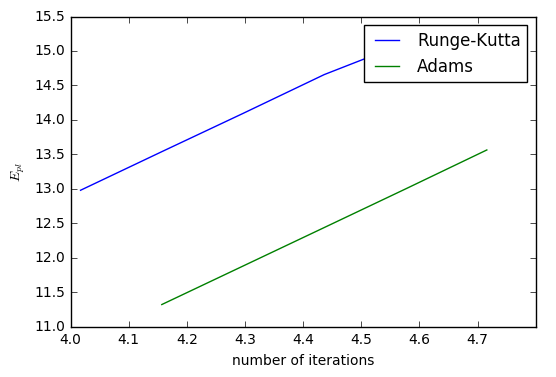
\includegraphics[scale=0.60]{imp-graph.png}
  \end{center}

\end{enumerate}
\end{document}
